\section{Approach}\label{sec:approach}

% Some tools for the latex code
\newcommand\Lb[1]{\mathit{Lb}(#1)}
\newcommand\InvLb[1]{\mathit{Lb}^{-1}(#1)}
\newcommand\Lbs[1]{\mathit{Lbs}(#1)}
\def\eqdef{\stackrel{\text{df}}{=}}
\newcommand\Hd[1]{\mathit{Head}(#1)}
\newcommand\HH[1]{\mathit{H}(#1)}
\newcommand\BB[1]{\mathit{B}^+(#1)}
\newcommand\BBn[1]{\mathit{B}^-(#1)}
\newcommand\Bd[1]{\mathit{Body}(#1)}
\newcommand\Bdp[1]{\mathit{Body}^+(#1)}
\newcommand\Bdn[1]{\mathit{Body}^-(#1)}
\def\eqdef{\stackrel{\text{df}}{=}}

\subsection{Syntax Scope and Grounder Simplifications}

%
\begin{itemize}
  \item
  We consider disyunctive ground logic programs with choice rules under the answer set semantics.
  %
  \item This is to avoid the simplifications that grounders do, which can be hard to track back to the original program.
  \item One of the reason for this simplifications is to have a simple normal form that can be interpreted by the solver.
  %
  \item This normal form allows disjunction or choices in the head, and either a sum aggregate with a lower bound or a conjunction of literals in the body.
  \cite{kamrom23a} \comment{S: perhaps there is a better reference for this? but I am not sure}
  \item To transform all available constructs in clingo into this normal form, the grounder introduces auxiliary atoms.
  \item This means that we will get auxiliary atoms when using
  $\#sum$ or $\#count$ aggregates, as well as
  anonymous variables,
  conditional literals,
  and choice rules with bounds or conditional literals within them.
  \item For instance, a choice rule written by the user as
  \item $1 \{ h;w \} 1\leftarrow a$ would be transformed into
  \begin{align*}
    aux\_0 &\leftarrow a \\
    \{ h;w \} &\leftarrow aux\_0 \\
    aux\_1 &\leftarrow 1\ \#sum\{1:h;\ 1:w\} \\
    aux\_2 &\leftarrow 2\ \#sum\{1:h;\ 1:w\} \\
    aux\_3 &\leftarrow aux\_1,\ \neg aux\_2 \\
    &\leftarrow\ aux\_0,\ \neg aux\_3
  \end{align*}
  \item In this case $aux\_0$ represents the body of the original choice rule,
  $aux\_1$ represents the lower bounds of the choice,
  $aux\_2$ represents the violation of the upper bound of the choice,
  $aux\_3$ represents the conjunction of the bounds,
  and the last rule is a constraint that ensures that if the body holds, then the bounds must hold as well.
  \item While one could provide meaningful names to some of these auxiliary atoms, we will not consider that analysis in this work.
  \item Furthermore, we do not consider sum aggregates, as this would require a more complex graph with weighted edges, and a special type of node to sum them up.

  %
\end{itemize}
%

\subsection{Labeled Logic Programs}

%
\begin{itemize}
  \item We refer to labelled logic programs because the program graph gives IDs to the bodies.
\end{itemize}
%

%
\paragraph{Labelled Ground Disjunctive programs}
A \emph{(labelled) rule} is an implication either of the form
\begin{eqnarray}
  \ell : p_1 \vee \dots \vee p_m \leftarrow q_1 \wedge \dots \wedge q_n \wedge \neg s_1 \wedge \dots \wedge \neg s_j \label{f:disjunctive-rule}
\end{eqnarray}
%
or of the form
%
\begin{eqnarray}
  \ell : \{p_1;\ \dots;\ p_m\} \leftarrow q_1 \wedge \dots \wedge q_n \wedge \neg s_1 \wedge \dots \wedge \neg s_j \label{f:choice-rule}
\end{eqnarray}
where $m, n, j \in \mathbb{N}_0$ (i.e., non-negative integers),
%
For any of the forms \eqref{f:disjunctive-rule} and \eqref{f:choice-rule}, we use $\Bd{r}$ and $\Hd{r}$ to refer to the \emph{antecedent} and the \emph{consequent} of the implication respectively.
%
We denote the set of atoms in the head of $r$ as
$\HH{r} \eqdef \{p_1, \dots, p_m\}$ in the case of rules of the form \eqref{f:disjunctive-rule}
and as $\HH{r} \eqdef \{a_1, \dots, a_k\}$ in the case of rules of the form \eqref{f:choice-rule}.
%
The set of atoms in the positive body are represented as
$\BB{r} \eqdef \{q_1,\dots,q_n\}$
and
the set of atoms in the negative body are represented as
$\BBn{r} \eqdef \{s_1,\dots,s_n\}$.
%
A \emph{(labelled) logic program} is a set of labelled rules.
%
Note that given any logic program $P$, we can get a labelled logic program by simply labelling each rule with an incremental identifier.
%
Given a rule $r$ like \eqref{f:disjunctive-rule} or \eqref{f:choice-rule}, we denote its label as $\Lb{r}\eqdef \ell$,
%
and so, we denote the rule $r$ corresponding to a label $\ell$ as $\InvLb{\ell}$.
%
Finally, we denote $\Lbs{P} \eqdef \{ \Lb{r} \mid r \in P \}$ as the set of all labels of the rules in a labelled program $P$.
\medskip
\comment{S: I think we should do all these as sets like $Dis(P)$ to be more consistent with the fact that we are defining many sets in this section, and have set operations below.}
%
$Dis(r)$: denotes that rule $r$'s head is a disjunction, that is, a rule of the form \eqref{f:disjunctive-rule}.
$Cons(r)$: denotes that a disjunctive rule $r$'s head is empty, that is, a constraint rule.
$Choice(r)$: denotes that rule $r$'s head is a choice, that is, a rule of the form \eqref{f:choice-rule}.
$Atoms(P)$ is the set of all the atoms occuring in $P$.
%

\paragraph{Open problems/questions}
\begin{itemize}
  \item
  {\color{red} We don't consider double negation.}
  TODO: to add a discussion somewhere in the paper on how this could affect
\end{itemize}

\subsection{Program Graph}

%
\begin{definition}[Program Graph]
%
Given a labelled logic program $P$, its \emph{program graph} is a directed graph
$G_P = \langle V_c \cup V_d \cup V_a, E_{+} \cup E_{-} \rangle$
where
%
$V_c$, $V_d$ and $V_a$ are nodes in the graph following the definitions below:
\begin{itemize}
    \item $V_d = \{ \Lb{r} \mid r \in P \land (Dis(r) \vee Cons(r))      \}$ is the set of rules's labels, whose head is a dijunction;
    \item $V_c = \{ \Lb{r} \mid r \in P \land Choice(r)    \}$ is the set of rules's labels, whose head is a choice;
    \item $V_a = \{ a      \mid a \in Atoms(P) \}$ is the set atoms which occur within any head of any rule in $P$.
\end{itemize}

and $E_{+}$ and $E_{-}$ are the sets of edges of the graph such that:
\begin{itemize}
  \item $\forall r \in P, \forall a \in \BB{r}  \rightarrow (a,\Lb{r})  \in E_{+}$
  \item $\forall r \in P, \forall a \in \BBn{r} \rightarrow (a, \Lb{r}) \in E_{-}$
  \item $\forall r \in P, \forall h \in \HH{r}  \rightarrow (\Lb{r}, h) \in E_{+}$
\end{itemize}
%
\end{definition}
%

%
\begin{example}[Program Graph]
  This is a modified version of the James Bond example from Fandinno
  \comment{TODO: look for the original reference}.
  A drug d in James Bond’s drink causes his paralysis p provided that he was not given an antidote a that day.
  We know that Bond’s enemy, Dr. No, poured the drug. He gets the antidote if he is not on holiday $h$.
  Unlike in the original example, we add $w$ to indicate a working day,
  and a choice to decide if James is on holiday or working,
  where the constraints in rules 2 and 3 ensuring exactly one of them is true.
  \comment{Note that adding the choice with bounds would have introduced auxiliary atoms as explained before, and would not be part of our restricted input.}
  %%
  \lstinputlisting[caption={Modified James Bond Example. Program $P_1$}, label={lst:example1}]{encodings/example1.lp}
  %%
  $P_1$ has two models, namely $M1 = \{w, d, a\}$ and $M2 = \{h, d, p\}$,
  where James is not poisoned in $M1$ since he is working and gets the antidote, and he is poisoned in $M2$ since he is on holiday and does not get the antidote.
  %
  Figure~\ref{fig:program-graph} shows the program graph corresponding to program $P_1$.
  \comment{TODO: match labels with $P_1$, also remove the natural language, also remove optional input}
  %
  \begin{figure}
    \centering
    % \includegraphics[width=0.75\textwidth]{resources/program-graph.png}
    % \includesvg[width=\textwidth]{resources/pg.svg}   %%% fails to scale text: asplain's or latex's problem?
    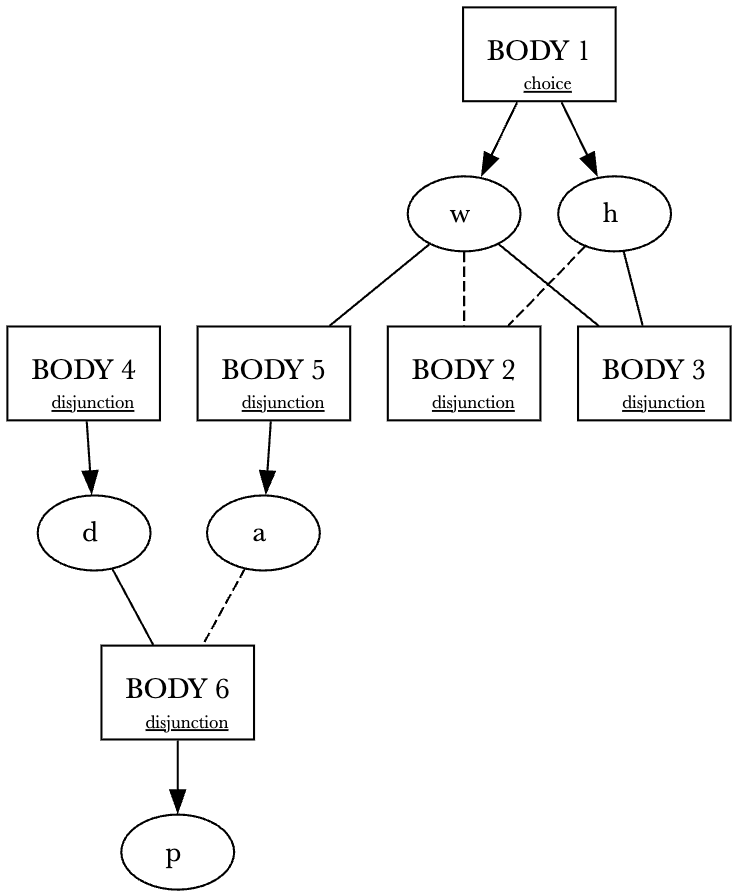
\includegraphics[width=0.5\textwidth]{resources/pg.png}
    \label{fig:program-graph}
    \caption{Program Graph $G_{P_{1}}$ corresponding to program in Listing~\ref{lst:example1}. }
  \end{figure}\comment{What do we do with optional nodes, that is abduction...}
  %
  Circle-nodes in graph $G_{P_{1}}$ represent atoms appearing in $P_1$, that is, the set $V_a = \{d,a,h,w,p\}$.
  %
  Rectangle-nodes in graph $G_{P_{1}}$ represent the body of some rule in $P_1$, in particular, sets $V_c = \{1\}$
  and $V_d = \{2,3,4,5,6\}$ correspond to the set of rules in $P_1$ whose head is a choice, respectively a disjunction.
  %
  Edges in $E^{+}$ are represented by solid arrows, while edges in $E^{-}$ are represented by dashed arrows.
  % For any atom (circle-node) $a \in V_c$ for which it exists some rule $r$
  % for which $a \in \HH(r)$, it must exist a solid edge $(r,a) \in E^{+}$.
  % %
  % For any atom (or circle-node) $a \in V_c$ for which it exists some rule $r$ for which $a \in \BB{r}$ (or respectively $a \in \BBn{r}$), it must exist a solid (respectively dashed) edge $(a,r) \in E^{+}$ (or respectively $(a,r) \in E^{-}$).
  % %

  %
  Note how, as expected, facts are depicted in the graphs as square nodes without any incoming edge, while constraints are depicted as square nodes without any outgoing edge.
  %
\end{example}

\begin{proposition}
  If two programs have the same program graph, they are strongly equivalent.
\end{proposition}


\paragraph{Discussion points}
\begin{itemize}
  \item
  $V_c$, $V_d$, $V_a$ are pairwise disjoint \comment{S: This would be simpler to show (I think) if the sets for Dis(r) is rather Dis(P)}
  \item
  A program graph is a directed graph that represents a logic program, in a solely syntactic way.

  \item
  We use this notion of graph as a basis for obtaining the explanations.

  \item
  It's intended to contain the full detail of what the ASP developer specified in the program.

  \item
  This notion its not intended to be used for the end-user, but we will see how to obtain user-oriented explanations from them once we have a answer set.

  \item
  As an additional advantage, this graph is easy to map back to clingo's metaprogramming features~\cite{kamrom23a}.
  That is, it resembles the meta program obtained by the grounder (gringo) from the original program.

  \item
  This notion will be useful for mappping different approaches to explanations in ASP.

  \item How to read the program graph \comment{Todo: CONNECT this with the sets/notation used}
  \begin{itemize}
    \item Circle nodes are atoms mentioned in the program.
    \item Box nodes are rule bodies. Note: after grounding aux rules are created for conditional literals, and others.
    \item Edges
    \begin{itemize}
      \item The graph is directed but directions are ommited so it must be read top-down. \comment{S: I think it might be best to add direction to all edges.}
      \item From rule (box) to atom (circle): atom is in the head of the rule
      \item From atom to rule: represent a literal. Positive when solid line, negative when dashed line.
    \end{itemize}
  \end{itemize}
\end{itemize}
%

\paragraph{Open problems/questions}
\begin{itemize}
  \item
  {\color{red} Doest it has a 1:1 relation with an ASP program?}.
  Should not be true for the \emph{orginal} program.
  \\
  But if the starter program is disyunctive and ground, then should be safe to say
\end{itemize}

\begin{proposition}
  Given two disyunctive, ground programs $P_1$ and $P_2$ and their respective program graphs $G_{P_1}$ and $G_{P_2}$, then
  \[ G_{P_1} = G_{P_2} \rightarrow P_1 = P_2 \]
\end{proposition}

\subsection{Model Subgraph}

\begin{definition}[Model Subgraph from Model]
  Given a program graph $G_P = \langle V_c \cup V_d \cup V_a, E_{+} \cup E_{-} \rangle$,
  and an answer set $I \subseteq V_a$ of $P$,
  a \emph{Model Subgraph} is a pair $MG_P^I = \langle V, E \rangle$ such that
  \begin{itemize}
    % take all the atoms in the model as nodes and all the supported rules as nodes as welll
    \item $V = I \cup \{ \Lb{r} \mid r \in P \land I \models \Bd{r} \}$
    % take all outgoing edges from atoms such that the corresponding (neg/pos) literal is supported by the model
    \item $\forall (a, \ell) \in E_{+}$ such that $a \in I$, then $(a, \ell) \in E$
    % \item $\forall (a, \ell) \in E_{-}$ such that $a \notin I$, then $(a, \ell) \in Em_{-}$   % we disregard the negative edges
    % take all outgoing edges from rules if the rule is supported by the model
    \item $\forall (\ell, a) \in E_{+}$ such that $I \models a \wedge \Bd{\InvLb{\ell}}$, then $(\ell, a) \in E$
  \end{itemize}
\end{definition}

%
\begin{proposition}
  Given a program $P$ and a model $I$ of $P$,
  the \emph{Model Subgraph} $MG_P^I$ is a subgraph of the \emph{Program Graph} $G_P$.
\end{proposition}
%
\begin{figure}
  \centering
  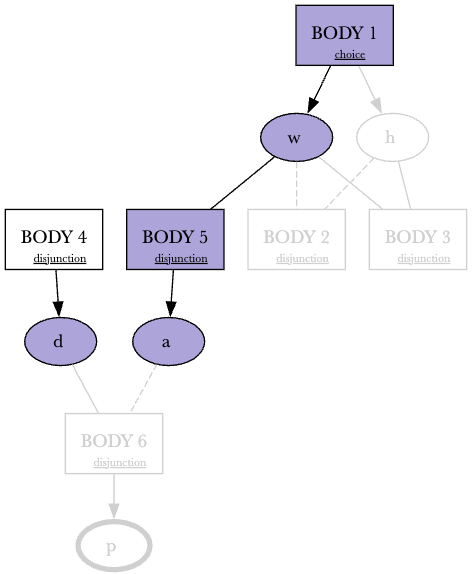
\includegraphics[width=0.5\textwidth]{resources/mask.png}
  \caption{Example of Model Subgraph.
  The entire program graph $G_{P_{1}} = \langle V_c \cup V_d \cup V_a, E_{+}\cup E_{-} \rangle$ can be seen, but the model subgraph $MG_{P_1}^{M1}$, which is highlighted  the answer set $M1 = \{w,a,d\}$.}
  \label{fig:model-mask}
\end{figure}


\paragraph{Discussion Points}
\begin{itemize}
  \item Intuition: we use a given model to extract a subgraph from the program graph, that highlights (1) supportiveness of atoms in the model; (2) supportiveness of rules; and (3) the truthness of the positive literals in the body.
  \item In our visualizations, we show the model subgraph coloured over the original program graph.
  \item How to read a Model Subgraph Visualizations.
  \begin{itemize}
    \item Atoms: cirlce node is colored if the corresponding atom is in the model.
    \item Literals: {\color{blue} only positive} literals are highlighted, in the form of the black, solid edges coming out of disjunctive and choice body, box-like, nodes.
    \item Rules: box node is colored if the body of the rule is supported by the model
    \item Derivations: black arrows going from bodies to atoms show that the atom could be derivated by that supported rule.
  \end{itemize}
  \item However, it {\color{blue} does not select any particular derivation} when alternative causes emerge (that is, is not causal) (is not equivalent to \cite{cabmun24a} but could be equivalent to \cite{altrsoba23a})
\end{itemize}

\paragraph{Discussion on having or not negative literals in the model subgraph}
  \begin{itemize}
    \item Since dashed edges represent negative literals, we could include them when the model does not support the literal.
    \item However, we can not include and edge that lacks its origin (breaks graph definition), so we would need to include the atom that is not in the model as well, which breaks the intuition of the model subgraph.
    \item Find below an enumeration of some types of explanations related to this, and if we can provide those answers without the negative literals in the \emph{model subgraph}. We need to discuss if we are interested on them or not.
    \begin{enumerate}
      \item For the rule $a \leftarrow b, not c$. With the model $\{ a, b\}$ we cannot answer \emph{a because b and not c}, because we do not include $c$ in the subgraph. We could however define an operation that use both the model graph and the program graph to do this.
      \comment{This is not what asplain is intended to do, but we can study this.}
      \item Answering \emph{a is not true because is not supported} is trivial and can be done.
      \item Considering the program
      \[
      \begin{array}{c}
        a \leftarrow body_1 \\
        a \leftarrow body_2 \\
        \dots               \\
        a \leftarrow body_n \\
      \end{array}
      \]
      answering \emph{$a$ is not true because $\neg body_1 \land \neg body_2 \land \dots \land \neg body_n$} cannot be answered by using a \emph{model subgraph} only (we do not have those bodies), but that conjunction can be obtained using the \emph{program graph} only.
    \end{enumerate}
    \item Latter type 3 however, lacks of some features that contrastive explanations give us. This is actually part of the motivation behind contrastive explanations:
    \begin{itemize}
      \item How a particular model interacts with some of the member of the conjunction $\neg body_1 \land \neg body_2 \land \dots \land \neg body_n$.
      \item How constraints in the proram interact with the conjunction, they could be prunning the scenarios where some of the $body_i$ holds.
      \item Preferences on which of the $body_i$ is more relevant (explnation preferences).
    \end{itemize}
  \end{itemize}

\begin{proposition}
  There should be a 1:1 correspondance between these model subgraphs and xASP explanations \cite{altrsoba23a} \comment{Son: xASP uses only one of the alternative for each atom, CHECK}
\end{proposition}


\subsection{Contrastive}

%       Extended version
% \paragraph{Context and Motivation}
% \begin{itemize}
%   \item Contrastivness is one of the main properties of human explanations~\cite{miller19}.
%   %
%   \item First, explanation-asking question (or queries) from humans are often contrastive, which means that they ask for some event that is not true in a world or scenario that is taken as reference.
%   %
%   \item To put an example, a typical human question/query would be \textit{Why isn't James posioned?}, implying a the existence of a scenario where James is not poisoned and that the asking human is taking as a reference.
%   %
%   \item In the real world, this reference world is normally a particular interpretation of the asking human about some events that she perceived.
%   %
%   \item A valid human contrastive explanation to that query will have to contrast the reference scenario with an alternative one where the question previously made is positively answered.
%   %
%   \item This alternative or hypothetical world is reffered in literature as \emph{foil}, whereas the reference world is reffered as \emph{fact}.
%   %
% \end{itemize}

%       Smaller version
\paragraph{Context and Motivation}
\begin{itemize}
  %
  \item Human explanations are often \emph{contrastive}~\cite{miller19}.
  %
  \item People ask “why not” questions relative to a reference and hypothetical/alternative scenarios.
  %
  \item Example: \textit{Why isn’t James poisoned?} — the asker \emph{assumes} or \emph{expects} a hypothetical world where James is poisoned.
  %
  \item This expectation is called \emph{foil} or \emph{foil world} in the literature, whereas the \emph{reference world} or \emph{fact world} is the asker’s interpretation of observed events where James is not poioned.
  %
  \item A contrastive explanation compares this \emph{reference world} with an \emph{foil world} where the outcome differs.
  %  %
\end{itemize}

\paragraph{Assumptions}
\begin{itemize}
  \item {\color{blue} We do not adress abduction here}, instead we just start from what is only neccesary to compute the contrastive graph.
  \item That is
  \begin{itemize}
    \item The program graph of the union of two programs $G_{P_r \cup P_f} = \langle V_c \cup V_d \cup V_a, E_{+}, E_{-} \rangle$ where $P_r$ and $P_f$ are the \emph{reference} and \emph{foil} programs, respectively.
    \item A \emph{reference model subgraph} $MG_{P_r}^{I_r} = \langle V_r, E_r \rangle$, for some $I_r$ such that $I_r \models P_r$
    \item The \emph{foil model subgraph} $MG_{P_f}^{I_f} = \langle V_f, E_f \rangle$, for some $I_f$ such that $I_f \models P_f$
    \item The query as set of literals $Q$.
  \end{itemize}
\end{itemize}

\begin{definition}[Existential Satisfaction]
  Given two sets of atoms $I_1$ and $I_2$ we say that they \emph{existentially satisfy} a term $t$, written
  \[ I_1,I_2 \models t \]
  iff:
  \begin{itemize}
    \item for a literal $l$ of the form $a$ or $\neg a$
    \begin{itemize}
      \item $I_1,I_2 \models a \iff a \in I_1 \vee a \in I_2$
      \item $I_1,I_2 \models \neg a \iff a \notin I_1 \vee a \notin I_2$
    \end{itemize}
    \item for sets of literals $B$
    \begin{itemize}
      \item $I_1,I_2 \models $B$ \iff I_1,I_2 \models l$ for every $l \in B$.
    \end{itemize}
    \item for a rule $r$ of the forms \eqref{f:disjunctive-rule} or \eqref{f:choice-rule}
    \begin{itemize}
      \item $I_1,I_2 \models r \iff I_1,I_2 \models \Bd{r}$
    \end{itemize}
  \end{itemize}
\end{definition}

\paragraph{Discussion on Existential Satisfaction}
\begin{itemize}
  \item Will be used to identify the conflict constraints among the masks used for a contrast.
  \item Is a very relax notion of satisfaction that can be read as \emph{this constraint would have been fired}.
\end{itemize}

\begin{definition}[Contrastive Subgraph]
  Given
  \begin{itemize}
    \item
    a set of literals $Q$ refered as \emph{query},
    \item
    two programs $P_r$ and $P_f$,
    \item
    a program graph $G_{P_r \cup P_f} = \langle V_c, V_d, V_a, E_{+}, E_{-} \rangle$,
    \comment{Problem? the labels of the rules in the programs might not coincide, so that if we do the union we might end up having repeated rules, different boxes. That's fine, in fact, we might want that. In labelled programs you sometimes want to have the same rule with different labels because they represent differnt knowledge sources.}
    \item
    a program subgraph $MG_{P_r}^{I_r} = \langle V_r, E_r \rangle$
    \item
    and
    a program subgraph $MG_{P_f}^{I_f} = \langle V_f, E_f \rangle$ such that $I_f \models Q$
  \end{itemize}
  then
  %
  a \emph{contrastive subgraph} is the tuple
  \[
  CM_{P_r, P_f}^{I_r, I_f} =
  \langle
    V_c, % 1. reference nodes, foil nodes, constraint nodes (or conflict nodes?)
    \langle E_c, E_{-} \rangle  % fact/foil positive edges, negative edges
  \rangle
  \]
  %
  where
  \begin{itemize}
    \item  $V_c = V_r \cup V_f \cup \{ \Lb{r} \mid (r \in P_r \cup P_f) \land (Cons(r)) \land (I_r, I_f \models \Bd{r}) \}$
    is the set of constraint nodes that are existentially satisfied by both reference and foil models

    \item $E_c = E_r \cup E_f$
    \item $E_{c-} = \{ (a, \ell) \mid (a, \ell) \in E_{-} \land [ (I_r \models a) \oplus (I_f \models a)]\}$
    we additionally add negative edges from the union program graph if that are satisfied by one world and not by the other.
  \end{itemize}
\end{definition}
\comment{Use the union of the two graphs instead? What do we do with the negative edges?}
%
\begin{proposition}
  Given a \emph{contrastive graph} $CM_{P_r, P_f}^{I_r, I_f}$,
  \begin{itemize}
    \item the \emph{model graph} $MG_{P_r}^{I_r}$ is a subgraph of $CM_{P_r, P_f}^{I_r, I_f}$
    \item the \emph{model graph} $MG_{P_f}^{I_f}$ is a subgraph of $CM_{P_r, P_f}^{I_r, I_f}$
    \item $CM_{P_r, P_f}^{I_r, I_f}$ is a subgraph of the \emph{program grpah} $G_{P_r \cup P_f}$.
  \end{itemize}
\end{proposition}
\comment{Might be so trivial}
%

%% contrastive
% pg1 --> model mask1 (all alternative justifications) --> causal mask1
% pg2 --> model mask2                                  --> causal mask2

% causal mask1 --> pg2 ?? % could be a distance function that ensures we keep as close as possible to the alternative chosen in causal mask1

% UnionGraph + causal mask1 + causal mask2 -->  Contrastive Graph  (asplain)
% UnionGraph + model mask1  + model mask2 -->  Contrastive Graph  (paper)

\paragraph{Discussion Points}
\begin{itemize}
  \item On top of the model subgraphs, the contrastive subgraphs give us two things:
  \begin{enumerate}
    \item Ensures that the contrast made answers the query $Q$.
    \item Uses both models to additionally hihglight \emph{constraint conflicts} and \emph{negative edges}.
  \end{enumerate}
\end{itemize}

\paragraph{Major Discussion on: Taxonomy/Types of Contrasts}
\begin{itemize}
  \item We may separate contrasts in types depending on the (dis)equalities among the programs $P_r$ and $P_f$, and the masks $MG_r$ and $MG_f$.
  \item We propose the following types
  \begin{itemize}
    \item when $P_r = P_f \land I_r = I_f$ then we call it \emph{positive justification}.
    \item when $P_r = P_f \land I_r \neq I_f$ then we call it \emph{alternative contrastive explanation}.
    \item when $P_r \neq P_f$ then we call it \emph{hypothetical contrastive explanation}.
  \end{itemize}
\end{itemize}



\subsection{Abduction for Contrastive Explanations}

\paragraph{Context and Motivation}
\begin{itemize}
  %
  \item Contrast is intended to be use to answer a user's query $Q$.
  %
  \item This query is something that do not hold in the reference world.
  %
  \item Abduction is the process we refer to find the \emph{foil world} that satisfies the query.
  %
  \item However, other processes could be used to find a valid \emph{foil world}, and we may study its relation with our notion of abduction.
  %
\end{itemize}

\paragraph{Assumptions}
\begin{itemize}
  %
  \item We start from a \emph{reference} program $P_r$ and a particular answer set $I_r$ of $P_r$.
  %
  \item Query $Q$ is a set of literals.
  %
  \item The process of \emph{abduction} is the process of finding a \emph{foil program} $P_f$ and an answer set $I_f$ of $P_f$ such that $I_f \models Q$.
  %
  \item The way we obtain $P_f$ and $I_f$ is by adding and removing rules from $P_r$ in a controlled way.
  %
\end{itemize}
%

%
\begin{definition}{Abducible programs}
  Given
  \begin{itemize}
    %
    \item a \emph{reference program} $P_r$,
    %
    \item a set of \emph{removable} labelled rules $R \subseteq P_r$ of the form \eqref{f:disjunctive-rule} and \eqref{f:choice-rule},
    %
    \item and
    %
    \item a set of \emph{addable} labelled rules $A$ of the form \eqref{f:disjunctive-rule} and \eqref{f:choice-rule},
    %
  \end{itemize}
  we denote $AP(P_r, A, R)$ as the set of all programs $P_f$ that satisfy
  \[
    P_r \setminus R \subseteq P_f \subseteq (P_r \cup A)
  \]
  Additionally, we say that $P_f$ is a valid \emph{abducible program from $P_r$ with respect to $A$ and $R$} if $P_f \in AP(P_r, A, R)$.
\end{definition}
%

%
\begin{definition}{Abducible Worlds}
  Given
  \begin{itemize}
    %
    \item a \emph{reference program} $P_r$,
    %
    \item a set of \emph{removable} labelled rules $R \subseteq P_r$ of the form \eqref{f:disjunctive-rule} and \eqref{f:choice-rule},
    %
    \item and
    %
    \item a set of \emph{addable} labelled rules $A$ of the form \eqref{f:disjunctive-rule} and \eqref{f:choice-rule},
    %
  \end{itemize}
  we denote $AW(P_r, A, R)$ as the set of all pairs $(P_f, I_f)$ satisfying
  \begin{itemize}
    \item $P_f \in AP(P_r, A, R)$
    \item $I_f \models P_f$
  \end{itemize}
  we call any of the pairs in the set as an \emph{abducible world from $P_r$}
\end{definition}
%
\begin{itemize}
  \item Note that we allow $P_r = P_f$
\end{itemize}
%

%
\begin{definition}[Valid Foil World]
  Given
  \begin{itemize}
    %
    \item a set of literals $Q$ refered as \emph{query},
    %
    \item a \emph{reference program} $P_r$,
    %
    \item a set of \emph{removable} labelled rules $R \subseteq P_r$ of the form \eqref{f:disjunctive-rule} and \eqref{f:choice-rule},
    %
    \item and
    %
    \item a set of \emph{addable} labelled rules $A$ of the form \eqref{f:disjunctive-rule} and \eqref{f:choice-rule},
    %
  \end{itemize}
  %
  we say the pair
  \[(P_f, I_f)\],
  is a \emph{valid foil world for $P_r$ with respect to $Q$} iff:
  \begin{itemize}
    \item $(P_f, I_f) \in AW(P_r, A, R)$
    \item $I_f \models Q$
  \end{itemize}
\end{definition}
%
\paragraph{Discussion}
\begin{itemize}
  %
  \item Regarding contrastive explanations, from a \emph{reference world} and a query $Q$, the idea is to find a valid foil world $(P_f, I_f)$ with with respect to $Q$, that will be later used to compute a \emph{model subgraph} $MG_{P_f}^{I_f}$, and then create a contrast graph $CG_{P_r, P_f}^{I_r, I_f}$.
  %
  \item {\color{blue} This definition does not impose the existence of a \emph{reference model} $I_r \models P_r$ neither that $I_r \nvDash Q$.} It's convenient as allow particular scenarios:
  \begin{itemize}
    \item \emph{unsat reference programs} $M(P_r) = \emptyset$ and $Q = \emptyset$, that is, we only want to recover satisfiability; or (b), $Q \neq \emptyset$, we want it to be sat and force something.
    \item When doing contrastive, the reference and foil models may collide $I_r = I_f$, which means that we are in fact doing no contrast. In other words, $I_r$ already satisfy the query.
  \end{itemize}

  %
  \item The sets $R$ and $A$ is what we informally call the \emph{abducibles}, that is, what we can add or remove to the original program in order to satisfy the query.
  %
  \item The most natural example of the abducibles is \emph{user input}, but any other notion can be abducible if it makes sense for the application.
  %
  \item The set $R$ (\emph{removables}) is only restricted to be a subset of $P_r$, while the set $A$ (\emph{addables}) is free, since we want to give full flexibility.
  %
  \item The idea is that they are defined for each use-case: the scope will be given as part of the domain, as user preference, as a programmer criteria, etc.
  %
  \item There exist two important sets that are not needed in the definition, those are:
  \begin{itemize}
    %
    \item $A_f = P_f \setminus P_r \subseteq A$, that is, the set of rules that were \emph{added}.
    %
    \item $R_f = P_r \setminus P_f \subseteq R$, that is, the set of rules that were \emph{removed}.
    %
    \item The role of $A_f$ and $R_f$ will probably take more importance when designing distances for implementing good explanation preferences.
  \end{itemize}
  %
\end{itemize}
%

\paragraph{Small Discussion on types of queries}
\begin{itemize}
  %
  \item The type of query is implicitly given by the satisfaction relation between $Q$ and $I_r$.
  \begin{itemize}
    %
    \item If $I_r \models Q$, then $Q$ is a \emph{Why query}. It does not require contrastive for being answered but our framework support this as a contrast as well (as mentioned earlier).
    %
    \item If $I_r \nvDash Q$, then $Q$ is a \emph{Why not query}, asking for contrastive explanation of $Q$ starting from $P_r$ and $I_r$ (and some sets $A$ and $R$).
  \end{itemize}
  %
  We do not answer in different ways depending on a taxonomy over a query. Queries are always sets of literals, and are answered always in the same way.
\end{itemize}


\subsection{Abduction Preferences}

\paragraph{Context and Motivation}
\begin{itemize}
  \item Since we provide full flexibility to find \emph{Foil Worlds}, we need to provide a way to select the appropiate one (or ones).
  \item In social sciences literature we see different notions of criteria on how to select the best \emph{foil world}: from the differences between the fact and foil worlds (the less the better), to other like temporal difference or probabilities.
  \item Other contrastive approaches, as \cite{eigeoe23a}, minimize the difference between both worlds or even require the minimals in that sense.
  \item We aim for a broader approach, by allowing to implement different criteria by defining a \emph{closeness function}.
  \item Examples of closeness functions:
  \begin{itemize}
    \item How many things have be removed/added.
    \item The differences between what is true and false in both models.
    \item Give preference to models that first remove things that were added interactively over input.
    \item ad-hoc distances for particular problems:
    \begin{itemize}
      \item In planning: defining a distance in terms of the cost of changing the plan.
    \end{itemize}
  \end{itemize}
\end{itemize}

\begin{definition}{Closeness Function}
  Given
  \begin{itemize}
    %
    \item a program $P_r$
    %
    \item a set of \emph{removable} labelled rules $R \subseteq P_r$ of the form \eqref{f:disjunctive-rule} and \eqref{f:choice-rule},
    %
    \item and
    %
    \item a set of \emph{addable} labelled rules $A$ of the form \eqref{f:disjunctive-rule} and \eqref{f:choice-rule},
    %
  \end{itemize},
  a \emph{closeness function} $cf$ is defined as
  \[
  cf : AW(P_r, A, R) \times AW(P_r, A, R) \to \mathbb{Z}
  \]
  that is, an application which maps a pair of two worlds from each program to an integer value.
\end{definition}

\paragraph{Disucssion on closeness function}
\begin{itemize}
  \item Intuitively, we start from the \emph{reference world} and a \emph{valid foil world} and we compute a numerical distance.
  \item We let the definition of the function open to each use case.
  \item {\color{red} ISSUE: This closeness function requires to provide a reference program-model pair, so it does not work when $P_r$ is unsat. Need to fix this.}
\end{itemize}

\begin{definition}[Closest Foil World]
  Given
  \begin{itemize}
    %
    \item a set of literals $Q$ refered as \emph{query},
    %
    \item a \emph{reference} program $P_r$,
    %
    \item a set of \emph{removable} labelled rules $R \subseteq P_r$ of the form \eqref{f:disjunctive-rule} and \eqref{f:choice-rule},
    %
    \item a set of \emph{addable} labelled rules $A$ of the form \eqref{f:disjunctive-rule} and \eqref{f:choice-rule},
    %
    \item Let $Foils(P_r, A, R, Q)$ be the set of all valid foil worlds $(P_f, I_f) \in AW(P_r, A, R)$ for $P_r$ with respect to $Q$.
    %
    and
    %
    \item  a valid \emph{closeness function} $cf$
    %
  \end{itemize}
  then
  the \emph{closest foil world for $P_r$ with respect to $Q$ and $cf$} is given by

  \[
  \mathrm{CFW}(P_r, A, R, Q;cf)
  := \argmin_{(P_f, I_f) \in Foils(P_r, A, R, Q)} \; cf(I_r, I_f).
  \]

\end{definition}




% \subsection{Relation to Support Graphs~\cite{cabmun24a}}
% %
% We refer back to~\cite{cabmun24a}, where the notion of \emph{support graph} or \emph{explanation} of an answer set with respect to a program is defined.
% %
% There, the nodes of the graph are only the atoms in the answer set, rules are not included as they are a technical detail of the program that might be hard to understand for the end-user.
% %
% The edges between the atoms, however, are obtained from the body of the rules in the program, connecting body literals with the the atoms in the head head and following some conditions.
% %
% Those conditions are used as the semantics for \emph{Justified Models}, whose relation with other approaches have been partly discussed in \cite{cabmun24a}.
% %
% Perhaps the most important condition is that the graphs have to \emph{select} one and only one rule to justify each atom in the answer set by defining an injective $\lambda$ function that maps each atom to the rule that justifies it.
% %
% Both an answer set of the program and the $\lambda$ function can be seen as a mask that can be applied on top of the program graph, obtaining a corresponding \emph{support graph}.
% %
% In~\cite{cabmun23a} two operations to select the relevant information within an explanation are introduced:
% first an operation to remove nodes, but preserving the transitive connection of the remaining nodes;
% and a second operation to prune edges, to remove non causal relations from the program.
% %
% We will use this two operations to obtain the all the corresponding support graph with respect to each answer set and a valid $\lambda$ function, from the program graph which is unique for each program.
% %
% However, in the case of the edge-prunning operation, it can be too weak for our purposes.
% %

% %
% \begin{definition}[Mask]
%   Given a program graph $G_P = \langle V_c \cup V_d \cup V_a, E_{+}, E_{-} \rangle$,
%   and an answer set $I \subseteq V_a$ of $P$,
%   an \emph{mask} of $G_P$ under $A$ is a function $\lambda: I \rightarrow V_c \cup V_d$ such that:
%   \begin{itemize}
%     \item $\lambda$ is injective {\color{blue} in $\lambda^{-1}(V_d)$}
%     \item $\forall a \in I, \lambda(a) = r \rightarrow I \models r$ \comment{TODO: allow non-injective mask for choice rules}
%     \comment{Note: We check cycles after inducing the subgraph.}
%   \end{itemize}
% \end{definition}
% %
% Notes:
% %
% \begin{itemize}
%   \item Intuitively, is a function that selects one supported rule for each atom in the answer set.
%   \item It can be applied to the program graph which gives us a subgrap that justifies each atom in the answer set.
% \end{itemize}
% %
% % \begin{definition}[Edges Mask]
% %   Given a program graph $G_P = \langle V_c \cup V_d \cup V_a, E_{+}, E_{-} \rangle$,
% %   and an answer set $I \subseteq V_a$ of $P$,
% %   an \emph{mask} of $G_P$ under $A$ is a function $\lambda: I \rightarrow E_{+}$ such that:
% %   \begin{itemize}
% %     % Lambda maps each atom to one of its incoming edges
% %     \item $\forall a \in I, \lambda(a) = (l, a) \land l \in E_{+}$
% %     % Disjunctive rules can only justify one atom
% %     \item $\forall a1, a2 \in I$ such that $\lambda(a1) = (l1, a1)$ and $\lambda(a2) = (l2, a2)$, then $l1 = l2 \rightarrow a1 = a2$.
% %     % The selected rule must be satisfied by the answer set
% %     \item $\forall a \in I, \lambda(a) = (l, a) \rightarrow I \models \InvLb{l}r$
% %     \comment{Note: We check cycles after inducing the subgraph.}
% %   \end{itemize}
% % \end{definition}
% %
% \begin{definition}[Edge Mask]
%   Given a program graph $G_P = \langle V_c \cup V_d \cup V_a, E_{+}, E_{-} \rangle$,
%   and an answer set $I \subseteq V_a$ of $P$,
%   a \emph{mask} of $G_P$ explaining $I$ is a set $EM \subseteq E_{+}$ such that:
%   \begin{itemize}
%     % There is an edge justifying each atom in the answer set such that the rule it comes from is satisfied by the answer set
%     \item $\forall a \in I, \exists (l, a) \in EM$ such that $I \models \InvLb{l}$.
%     % If a rule is used to satisfy an atom, then all its incoming edges are in the mask
%     \item $forall (l, a) \in EM$, such that $I \models \InvLb{l}$, then $\forall (a', l) in E_{+}$ it must hold that $(a', l) \in EM$.
%     % Only one incoing edge per atom
%     \item $\forall  (l1, a1),(l2, a2) \in EM$, it must hold $(a1 = a2) \rightarrow (l1 = l2)$
%     % Disjunctive rules can only justify one atom
%     \item $\forall (l1, a1),(l2, a2) \in EM$, it must hold $(l1 = l2) \land (l1 \in V_d) \rightarrow (a1 = a2)$.
%   \end{itemize}
% \end{definition}
% %
% Notes:
% %
% \begin{itemize}
%   \item A mask then would be a subset of edges of the program graph that selects one edge for each atom in the answer set.
%   \item This alternative definition of mask may better fit the current implementation.
%   \item It's equivalent to the previous.
% \end{itemize}
% %

% %
% \begin{definition}[Answer Set Explanation Graph]
%   Given a program graph
%   $G_P = \langle V_c \cup V_d \cup V_a, E_{+}, E_{-} \rangle$,
%   corresponding to a ASP program $P$,
%   and an answer set $I \subseteq V_a$ of $P$,
%   and a \emph{mask} $\lambda: I \rightarrow V_c \cup V_d$ of $G_P$ under $I$,
%   an explanation of $I$ under $P$ is a directed graph
%   \[    G_{\lambda} = \langle V, E \rangle    \]
%   where:
%   \begin{itemize}
%     \item $V = I \cup Im(\lambda)$
%     \item $E = \{ (\ell, a) \in E_{+} \mid \lambda(a) = \ell \} \cup \{ (a, \ell) \in E_{+} \mid \ell \in Im(f) \}$
%     \item {\color{red} There is no cycles in $G_{\lambda}$.}
%   \end{itemize}
% \end{definition}
% %
% Notes:
% \begin{itemize}
%   \item Intuitively, this graph is a subgraph of the support graph, where we only keep the nodes in the answer set and the rules that justify them following a particular $\lambda$.
%   \item It only contains positive edges.
%   \item Find an example of a mask and the corresponding answer set explanation in Figure~\ref{fig:mask}.
%   \item For any answer set $I$ of a program $P$ there is always at least one mask $\lambda$ such that the technical explanation $G_{\lambda}$ is a directed acyclic graph (DAG) (pontentially many). \comment{I have to prove this by proving the correspondance with Justified Models.}
%   \item In Figure~\ref{fig:mask}, note that there is another mask $\lambda_2$ for explaining $M_1$ that justifies the atom $a$ with rule $5$, that is $\lambda_2(a) = 5$.
% \end{itemize}
% %
% \begin{definition}[Answer Set Explanation Graph with Edges Mask]
%   Given a program graph
%   $G_P = \langle V_c \cup V_d \cup V_a, E_{+}, E_{-} \rangle$,
%   corresponding to a ASP program $P$,
%   and an answer set $I \subseteq V_a$ of $P$,
%   and a \emph{edge mask} $EM \subseteq E_{+}$ explaining $I$,
%   an explanation of $I$ under $P$ is a directed graph
%    \[    G_{EM} = \langle V, EM \rangle    \]
%   where
%   % v is any origin or destination of an edge in $EM$
%   $V = \{ v \mid \exists (v, w) \in EM \vee \exists (w, v) \in EM \}$
% \end{definition}
% %

% %
% \begin{figure}
%   \centering
%   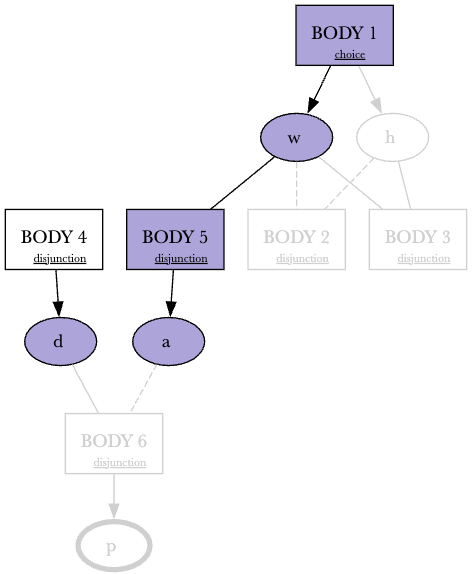
\includegraphics[width=0.9\textwidth]{resources/mask.png}
%   \caption{Mask.
%   The entire program graph $G_{P_{1}} = \{V_c, V_d, V_a, E_{+}, E_{-}\}$ can be seen, but the highlighted part of the graph explains the answer set $M_1 = \{s,w,a,d\}$.
%   This subgraph is the techincal explanation $G_{\lambda} = \langle V, E \rangle$ induced from a mask $\lambda: M_1: \rightarrow $ where $\lambda(s) = 1$, $\lambda(w) = 4$, $\lambda(a) = 2$ and $\lambda(a) = 3$.}
%   \label{fig:mask}
% \end{figure}
% %

% {\color{gray}
% %
% \begin{definition}[Technical Non-Causal Explanation]
%   Given a program graph
%   $G_P = \langle V_c \cup V_d \cup V_a, E_{+}, E_{-} \rangle$,
%   corresponding to a ASP program $P$,
%   and an answer set $I \subseteq V_a$ of $P$,
%   and an injective function $\lambda: I \rightarrow V_c \cup V_d$ such that selecting a rule $r$ such that $I \models r$ to justify each atom,
%   a techincal explanation of $I$ under $P$ is a directed graph
%   \[    G_t = \langle V_{+}, V_{-}, E_{t}^{+}, E_{t}^{-} \rangle    \]
%   where:
%   \begin{itemize}
%     \item $V_{+} = I \cup Im(\lambda)$
%     \item $V_{-} = \bigcup_{l \in Im(\lambda)}{\Bdn{\InvLb{l}}}$
%     \item $E_{t}^{+} = \{ (\ell, a) \in E_{+} \mid \lambda(a) = \ell \} \cup \{ (a, \ell) \in E_{+} \mid \ell \in Im(\lambda) \}$
%     \item $E_{t}^{-} = \{ (a, \ell) \in E_{-} \mid \ell \in Im(\lambda) \land a \in \Bdn{\InvLb{l}} \}$
%     \item {\color{red} There is no cycles in $G_t$.}
%   \end{itemize}
%   %
%   \comment{TODO: this version is intended to be used for correspondance with xASP, left for future work}
% \end{definition}
% %
% \begin{figure}
%   \centering
%   \includegraphics[width=0.9\textwidth]{resources/tech-non-causal.jpg}
%   \caption{Technical Non Causal Explanation}
%   \label{fig:gt_noncausal}
% \end{figure}
% }
% %


% % % TODO: the correspondance
% % Moreover, a proper support graph is obtained by applying the node forgetting operation to the technical explanation, effectively removing any rule referencing node and keeping only nodes referencing atoms.
% % %
% % That is $G = forget(G^t, V_c \cup V_d)$.
% % %
% % \begin{proposition}
% %     Let $G_{P} = \{V_c, V_d, V_a, E_{+}, E_{-}\}$ be the program graph for program $P$,
% %     and a mask \lambda $G_{\lambda} = \langle V_t, E_t \rangle$ be a causal technical explanation of an answer set $I$ under a program $P$,
% %     then graph $G^s = forget(G_{\lambda}, V_c \cup V_d)$ is a valid support graph of $I$ under $P$.
% % \end{proposition}
% % %

% % %
% % In~\cite{cabmun24a} support graphs are introduced as a way to globally explain a particular answer set of a program.
% % %
% % Then, authors explain how to obtain \emph{local explanaitions} or \emph{proofs} for particular atoms from the suppport graph.
% % %
% % This is done by recursively traversing the graph backwards from the explained atom.
% % %
% % It is trivial to see how this can also be done from the technical explanation although this time the obtained \emph{tree} or \emph{proof} will also include the rule nodes.
% % %


\section{Implementation}

\paragraph{Motivation}
\begin{itemize}
  \item To match the implementation and to prove that it is correct with respect to our definitions.
\end{itemize}

\subsection{Program Graph Semantics: Finding Models (Masks)}
\begin{definition}[Classical Model Mask]
  Given a program graph $G_P = \langle V_c \cup V_d \cup V_a, E_{+}, E_{-} \rangle$,
  a subgraph $CM = \langle Vm, Em_{+}, Em_{-} \rangle \subseteq G_P$ is a \emph{classical model mask} of $G_P$
  iff:
  \begin{itemize}
    \item
    $Vm =
      % take the boxes for which we already have all the incoming edges (facts are trivial)
      \{ \ell \in V_c \cup V_d \mid \forall (a,\ell) [(a,\ell) \in E_{+} \rightarrow (a,\ell) \in Em{+}] \} \cup
    $
    \item $Em_{+} = Em_{+} \cup C_{hoices} \cup \bigcup_{i=1}^{n} A_i
    $

  \begin{itemize}
              % For any choice box already in the graph, take any subset of its outgoing edges
    \item where $C_{hoice} \subseteq \{ (\ell, a) \mid \ell \in Vm \land (\ell, a) \in E_{+} \}$
  \end{itemize}
\end{itemize}

\end{definition}
\comment{Map the program from how to build your own asp system and Susana's}

\begin{definition}[(minimal) Model Mask]
  Given a program graph $G_P = \langle V_c \cup V_d \cup V_a, E_{+}, E_{-} \rangle$,
  we say a valid \emph{classical model mask} $CM = \langle V, E_{+}, E_{-} \rangle$ of $G_P$
  is a \emph{(minimal) Model Mask} $MG$ of $G_P$
  iff
  \begin{center}
    $MG$ is $\subseteq-minimal$ among all the \emph{classical model masks} of $G_P$.
  \end{center}
\end{definition}
\comment{Map the program from how to build your own asp system and Susana's}


\comment{S: Given a program graph we can also compute the models. I think this should be made clear somewhere, this is just a sketch, I am not sure how to write it.}
\begin{definition}[Model Subgraph Computed]
  Given a program graph $G_P = \langle V_c \cup V_d \cup V_a, E_{+} \cup E_{-} \rangle$,
  a \emph{Model Subgraph} is a pair $MG_P^I = \langle V, E \rangle$ such that
  \begin{itemize}
    % Body satisfaction
    \item for any $\ell\in V_d\cup V_c$,
    if $a\in V$ for all $(a, \ell) \in E_{+}$
    and $a\not\in V$ for all $(a, \ell) \in E_{-}$,
    then $\ell \in V$.

    % Atom satisfied by disjunction
    \item for all $\ell\in V_d\cap V$ then for (exactly one) $(\ell,a) \in E_{+}$ happens $a\in V$.

    % Atom satisfied by choice
    \item for all $\ell\in V_c\cap V$ then for any $(\ell,a) \in E_{+}$, $a\in V$ is optional.


  \end{itemize}
\end{definition}


\paragraph{Discussion points}
\begin{itemize}
  \item This is how asplain collect the model masks
  \item Since the model masks are computed, we mimic the asp semantics, we first go for the classical models and then get the minimal ones.
\end{itemize}



% \subsection{Whynot queries}

% %
% Three different concepts:
% \begin{itemize}
%     \item \textbf{Natural language question}:
%     %
%     human users express they information needs in natural language.
%     %
%     It's inherently ambiguous and the same expression can be interpreted in many ways, that is, the relation between an expression and a formalized query it's $N:N$.
%     %
%     \item \textbf{Query}:
%     %
%     a formal/mathematical object that encodes an infromation need.
%     %
%     Dependant of the system.
%     %
%     \item \textbf{Answer}:
%     %
%     deterministic and replicable with respect to the query and system.
%     %
%     It fulfils the information need of the original natural language question.
%     %
% \end{itemize}

% %
% From social sciences~\cite{miller19} we know that human explanations are:
% %
% \begin{enumerate}
%     \item \textbf{Selected}:
%     %
%     a good explanation only include the relevant information and exclude irrelevant details.
%     %
%     This filter is highly relative to the persons involved and their contexts which connects with point 2.
%     %
%     \item \textbf{Social}:
%     %
%     in an explanation, we have at least two involved entities: the \emph{explainer} and the \emph{explainee}.
%     %
%     In our case, asplain and the user respectively.
%     %
%     The explanation is always \emph{social interaction}, even if one of the entities is a non-human system.
%     %
%     As a social interaction, it's highly dependant of the context, and the entities's contexts.
%     %
%     Naturally, the contents (what info is included/excluded) and the form (language, tone, extension, etc.) of the explanation are set by the \emph{explainer}.
%     %
%     But in the case of humans, the explainer is able to \textbf{adapt} both to the \emph{explainee} context.
%     %
%     For instance, when explaining the reasons behind the disease of a patient, the doctor (\emph{explainer}) will not provide the same explanation to her colleges than to the patient.
%     %
%     This adjustments include the language (which words are chosen), the tone, the length but also which info is included/excluded and the importance given to each piece of information (this could even affect the order the information is presented, but we are not controlling that in asplain).
%     %
%     \item \textbf{Contrastive}:
%     %
%     this point mainly speaks about which type of queries humans often ask, and how do they ask them.
%     %
%     We can synthetise this in two points.
%     \begin{itemize}
%         \item \textbf{Most queries are a ''why not´´}:
%         %
%         humans often ask for an explanation when they are surprised by an unexpected event and ask for explanation of why their expectations weren't fulfilled.
%         %
%         That is, the \emph{explainee} pressuposes a world / expects an outcome / has a mental model (from now on the \emph{default world}) that is broken by the real events (that Miller refers to as \emph{fact}, and we as the \emph{reference world}).
%         %
%         For instance, let's say that Q goes to visit James Bond expecting him to be fine, only to find out that he died poisoned.
%         %
%         There, Q asks \emph{Why did James died poisoned?} or \emph{\textbf{Why} is \textbf{not} James alive?}.
%         %
%         According to Miller, both questions actually map to the same query \textbf{Why not alive} since, disregarding how Q formulated his information need in natural language, what is important what was assumed by Q's default world (James should have been alive).
%         %
%         Human
%         %

%         %
%         This does not apply to the 100\% of the questions made by humans,
%         %

%     \end{itemize}
%     %

%     %
%     \item \textbf{Causal}:
% \end{enumerate}
% %

% \subsection{Contrastive explanations}

% \begin{itemize}
%     \item A contrastive explanation compares a reference model to a contrasted model.
%     \item It can cover also cases for justifying something that is true in the model.
%     So it might subsume other types of explanations that are only causal.
%     \item Can be formalized as a graph.
%     But has to add a lot of information into the edges and nodes.
%     \item \textbf{Query:} Identifies what atoms should/shouldn't be part of the model.
%     \item \textbf{Reference model:}
%     The provided model that is considered the current truth.
%     \item \textbf{Contrasted model:}
%     The model found which fulfils the query.
%     \begin{itemize}
%         \item \textbf{Same as reference model}
%         When the query is true in the current model, then the contrasted and reference model are the same.
%         The output is something like the current output of xclingo or ucorexplain\cite{alhasawe24a}.
%         \item \textbf{Alternative model}
%         When the query is not true in the current model but it is true without having to change the input (no abducible needed).
%         This is the case where another model of the same program (with the same input) satisfies the query.

%         The explanation would compare both models without need of abduction.
%         \item \textbf{Hypothetical model}
%         When the query can't be satisfied with the current input
%         Parts of the input can be abducted (changed) to achieve the query
%     \end{itemize}
% \end{itemize}


% \begin{definition}[Contrastive Explanation (preliminary)]
%     Let $P_{ref}$ and $P_{alt}$ be two labelled logic programs,
%     $I_{ref} \in CM(P_{ref})$ and $I_{alt} \in CM(P_{alt})$ be two classical models of $P_{ref}$ and $P_{alt}$ respectively,
%     let
%     $G_{ref} = \langle I_{ref}, E_{ref}, \lambda_{ref} \rangle$ be a support graph explanation of $I_{ref}$ with respect to $P_{ref}$,
%     and
%     $G_{alt} = \langle I_{alt}, E_{alt}, \lambda_{alt} \rangle$ be a support graph explanation of $I_{alt}$ with respect to $P_{alt}$.


%     A \emph{contrastive explanation graph} is a tuple:
%     \[
%     G = \langle V, \lambda_{ref}, \lambda_{alt}, E^c, E^i \rangle
%     \]
%     where:
%     \[
%     V  = I_{ref} \cup I_{alt} \cup \{ \lambda_{ref}(r) \mid r \in \text{CONSUP}(P_{ref}, I_{ref}, I_{alt}) \}
%     \],
%     \begin{align*}
%         E^c = {} &
%         E_{ref} \cup E_{alt}\\
%         & \cup
%         \left\{
%           (con, r) \in V \times V \mid
%           \begin{array}{l}
%             r \in CONSUP(P_{ref}, I_{ref}, I_{alt}), \\
%             con \in B^+(r) \\
%             con \in I_{ref} \cup I_{alt}
%           \end{array}
%         \right\}
%     \end{align*}
%     \begin{align*}
%         E^i = {} &
%         \left\{
%           (i, e) \in V \times V \mid
%           \begin{array}{l}
%             e \in I_{ref} \setminus I_{alt},
%             i \in I_{alt} \setminus I_{ref}, \\
%             \lambda_{ref}(e) = Lb(P_{ref}, r), \\
%             r \in SUP(P_{ref}, I_{ref}, e), \\
%             i \in B^-(r)
%           \end{array}
%         \right\} \\
%         & \cup
%         \left\{
%           (i, e) \in V \times V \ \mid
%           \begin{array}{l}
%             e \in I_{alt} \setminus I_{ref},
%             i \in I_{ref} \setminus I_{alt}, \\
%             \lambda_{alt}(e) = Lb(P_{alt}, r), \\
%             r \in SUP(P_{alt}, I_{alt}, e), \\
%             \text{not } i \in B^-(r)
%           \end{array}
%         \right\} \\
%         & \cup
%         \left\{
%           (con, r) \in V \times V \mid
%           \begin{array}{l}
%             r \in CONSUP(P_{ref}, I_{ref}, I_{alt}), \\
%             \text{not } con \in B^-(r) \\
%             con \notin I_{ref} \cap I_{alt}
%           \end{array}
%         \right\}
%     \end{align*}
%     % \[
%     % E^{c}_{con} = {} &
%     %     \left\{
%     %       (con, r) \in V \times V \mid
%     %       \begin{array}{l}
%     %         r \in CONSUP(P_{ref}, I_{ref}, I_{alt}), \\
%     %         con \in B^+(r) \\
%     %         con \in I_{ref} \cup I_{alt}
%     %       \end{array}
%     %     \right\}
%     % \]
%     % \[
%     % E^{i}_{con} = {} &
%     %     \left\{
%     %       (con, r) \in V \times V \mid
%     %       \begin{array}{l}
%     %         r \in CONSUP(P_{ref}, I_{ref}, I_{alt}), \\
%     %         \text{not } con \in B^-(r) \\
%     %         con \in I_{ref} \triangle I_{alt}
%     %       \end{array}
%     %     \right\}
%     % \]

% \end{definition}


% % \begin{definition}[Contrastive Explanation]
% %     Let $P_{ref}$ and $P_{alt}$ be two labelled logic programs,
% %     $I_{ref} \in CM(P_{ref})$ and $I_{alt} \in CM(P_{alt})$ be two classical models of $P_{ref}$ and $P_{alt}$ respectively,
% %     let
% %     $G_{ref} = \tuple{I_{ref}, E_{ref}, \lambda_{ref}}$ be a support graph explanation of $I_{ref}$ with respect to $P_{ref}$,
% %     and
% %     $G_{alt} = \tuple{I_{alt}, E_{alt}, \lambda_{alt}}$ be a support graph explanation of $I_{alt}$ with respect to $P_{alt}$.


% %     A \emph{contrastive explanation graph} is a tuple:
% %     \[
% %     G = \tuple{V, \lambda_{ref}, \lambda_{alt}, E^c, E^i, E^{con}}
% %     \]
% %     where:
% %     \[
% %     V  = I_{ref} \cup I_{alt}
% %     \],
% %     \begin{align*}
% %         E^c = {} &
% %         E_{ref} \cup E_{alt}\\
% %         & \cup
% %         \left\{
% %           (con, r) \in V \times V \mid
% %           \begin{array}{l}
% %             r \in CONSUP(P_{ref}, I_{ref}, I_{alt}), \\
% %             con \in B^+(r) \\
% %             con \in I_{ref} \cup I_{alt}
% %           \end{array}
% %         \right\}
% %     \end{align*}
% %     \begin{align*}
% %         E^i = {} &
% %         \left\{
% %           (i, e) \in V \times V \mid
% %           \begin{array}{l}
% %             e \in I_{ref} \setminus I_{alt},
% %             i \in I_{alt} \setminus I_{ref}, \\
% %             \lambda_{ref}(e) = Lb(P_{ref}, r), \\
% %             r \in SUP(P_{ref}, I_{ref}, e), \\
% %             i \in B^-(r)
% %           \end{array}
% %         \right\} \\
% %         & \cup
% %         \left\{
% %           (i, e) \in V \times V \ \mid
% %           \begin{array}{l}
% %             e \in I_{alt} \setminus I_{ref},
% %             i \in I_{ref} \setminus I_{alt}, \\
% %             \lambda_{alt}(e) = Lb(P_{alt}, r), \\
% %             r \in SUP(P_{alt}, I_{alt}, e), \\
% %             \text{not } i \in B^-(r)
% %           \end{array}
% %         \right\}
% %     \end{align*}
% %     \begin{align*}
% %         E^{con} = {} &
% %         \left\{
% %           (c2, c1) \in V \times V \mid
% %           \begin{array}{l}
% %             r \in CONSUP(P_{ref}, I_{ref}, I_{alt}), \\
% %             \text{not } con \in B^-(r) \\
% %             con \notin I_{ref} \cap I_{alt}
% %           \end{array}
% %         \right\}
% %     \end{align*}
% % \end{definition}

% \begin{itemize}
%     \item $CONSUP(P,I_1,I_2,R) \stackrel{\text{df}}{=} \{r \in P \mid Head(r) = \bot \land \forall \text{lit } \in Body(r), I_1 \models \text{lit } \vee I_2 \models \text{lit }\}$
%     \item A contrastive explanation answers a query $Q$ if $I_{alt} \models Q$
%     \item (abduction) Given two sets of facts: $Add$ and $Rm$. $P_{alt}$ is obtained by considering subsets $A \subseteq Add$ and $R \subseteq Rm$ such that: $P_{alt} = (P_{ref} \setminus R) \cup A$. $A = R  \rightarrow P_{alt} = P_{ref}$, that is, no abduction was needed (alternative explanation).
%     \begin{itemize}
%         \item \textbf{why} queries. When $I_{ref} = I_{alt}$ and $P_{ref} = P_{alt}$ ($A = R$ and possibly $A = R = \emptyset $) and $\lambda_{ref} = \lambda_{alt}$, the query is true in the reference model.
%         \item \textbf{whynot} contrastive (non counterfactual, alternative). When $P_{ref} = P_{alt}$ and $I_{ref} \neq I_{alt}$
%         \item \textbf{whynot} contrastive and counterfactual (hypothetical). When $P_{alt} \neq P_{ref}$ and $I_{ref} \neq I_{alt}$.
%     \end{itemize}
%     \item
%         IMPORTANT: constraints are only got from reference model.
%         Does it makes sense to add constraints in the hypothetical world?
%         Maybe to select hypothetical worlds. Like: in the query we could say "never abduce this and this".
%         But, never for explanation, as introducing constraints in $P_{alt}$ only prunes $P_{ref}$ models which never helps in satisfying queries.
% \end{itemize}

% \begin{definition}[Asplain's Contrastive Explanation]
%     Define a function that takes a Contrastive Explanation and
%     \begin{itemize}
%         \item Hides nodes (constraint nodes are always hidden)
%         \item Prunes edges.
%         \item \textbf{Enablers may now appear}
%     \end{itemize}
% \end{definition}

% \begin{definition}[Using only reachability]
%     \item Using the defined function
%     \item Reverse traverse the graph from the
% \end{definition}

% \subsection{Selecting the contrasted model}

% \begin{itemize}
%     \item Notice that the minimization we might impose is not subset minimal like for MUS.
%     The subset minimality can't be encoding in ASP directly.
%     \item We can think of this selection as explanation preferences that define the contrastive model.
%     This preference can be encoded in an ASP program.
%     At the moment this is very general, since we use any program\comment{TODO: how do we formalize this?}
%     \item We don't see so many papers talk about preferences on explanations.
%     In \cite{alhasawe24a}  there is the option to move up and down rules to prefer some more than others, but that is it. \comment{TODO: Check if this is really the case}

% \end{itemize}


% \subsubsection{Abducibles}


% \begin{itemize}
%     \item Things that will change from the reference model to the hypothetical one.
%     They can be either added or removed in the contrasted model.
%     \item The possible atoms to abduce are defined for each application.
%     \item There is a difference between abducing a predicate in the whole program,
%     which means that even if it comes from a rule, if it is abduced then it wont be generated,
%     vs an option where only the facts are abduced. This boils down to the question of abducing rules vs abducing facts.
%     \item What is abducible or not is defined by the \emph{explanation-preference} ASP program.
%     Depending on what is abducible we may be giving different types of explanations/answers.
%     For instance: in the case of an reasoning agent, it does not make sense to abduce thing that were observed, but only beliefs or possible actions.
%     Similar in the case of diagnosis.
%     For sudoku or configuration, it does makes sense to abduce the user's input.
% \end{itemize}

% \subsection{Implementation}\label{sec:approach:implementation}

% \begin{itemize}
%     \item We use several transformers to create new rules and add information. \comment{TODO: Perhaps part of this can be done with clingos reification?}
%     \item The intention is to also make this Transformers available for future explanation tasks. \comment{TODO: Where do we want to make this available? clingoexplaid?}
%     \item The explanation preference is encoded as an additional ASP encoding.
%     \item The contrastive graph is defined as a set of facts. Where attributes on edges and nodes give the contrastive semantics.
%     \item We give the full graph, although the relevant information for the query might be in just one part.
%     Creating a reduced reachable graph is possible, but we will try to leave this to the LLM.
%     \item Accepted language fragment \comment{TODO: Brais is adding count}
%     \item Facts defining the contrastive graph:


%         \begin{itemize}
%             \item \texttt{node(A)}: Defines a node in the graph
%             \begin{itemize}
%                 \item \textbf{A}: the node identifier (atom)
%             \end{itemize}
%             \item \texttt{edge(N,N',ID)}: Defines an edge in the graph. They represent the causal relationships between nodes, as well as negative relationships (inhibitors).
%             \begin{itemize}
%                 \item \textbf{N}: the origin node
%                 \item \textbf{N'}: the destination node
%                 \item \textbf{ID}: the identifier of the edge (Required for multi-edges)
%             \end{itemize}
%             \item \texttt{attr(T,N,A,V)}: Defines an attribute for a node or edge.
%             \begin{itemize}
%                 \item \textbf{T}: the type of the element (\texttt{node} or \texttt{edge})
%                 \item \textbf{N}: the node or edge identifier
%                 \item \textbf{A}: the attribute name
%                 \item \textbf{V}: the attribute value
%             \end{itemize}
%             \begin{itemize}
%                 \item \textbf{T=\texttt{node}}:
%                 \begin{itemize}
%                     \item \texttt{A=origin}: \texttt{V} = either \texttt{real} or \texttt{hypothetical}
%                     \item \texttt{A=abduced}: \texttt{V} = either \texttt{rm} or \texttt{add}
%                     \item \texttt{A=query}: \texttt{V} = either \texttt{include} or \texttt{exclude}
%                 \end{itemize}
%                 \item \textbf{T=\texttt{edge}}:
%                 \begin{itemize}
%                     \item \texttt{A=origin}: \texttt{V} = either \texttt{real} or \texttt{hypothetical}
%                     \item \texttt{A=type}: \texttt{V} = either \texttt{inhibitor} \texttt{reciprocal\_inhibitor} or \texttt{cause}
%                 \end{itemize}
%             \end{itemize}
%         \end{itemize}
% \end{itemize}

% \subsection{Interactivity}

% \begin{itemize}
%     \item We can integrate this system into an interactive setting where we make a difference between user selections and input.
%     \item In this case we can change the explanation preference encoding, to prefer abducing user input before the input for the problem.
%     For instance, in a sudoku, you would first say that in order to put a 1 in a cell you would have to change the 1 you put on that road,
%     rather than saying that there would have to have to change the 1 that was an initial input value somewhere else, which the user can't change themselve.
% \end{itemize}


% \subsection{LLM}

% \begin{itemize}
%     \item We use the LLM to interpret our graph into natural language.
%     \item Do we want to use also the LLM to generate the query atoms? Like in \cite{gekaoe24a}?
%     \item The only input for the LLM is the computed graph as facts.
%     \item The LLM could have a more structured output, like a JSON structure that gives more information.
%     For instance, the atoms that are relevant for the natural language explanation provided.
%     This would be useful in a system like clinguin to highlight sections of the UI.
% \end{itemize}


